\section{Lecture 13: 23.09.2025}

\subsection{Convergence properties of GMRES (Generalized Minimal Residual Method)}
\begin{itemize}
    \item $\mathbf{x}_\star$ exact solution of $A\mathbf{x} = \mathbf{b}$.
    \item $\mathbf{x}_m$ numerical solution after $m$ iterations with some \emph{krylov-space method}.
          \[
              \mathbf{r}_m = \mathbf{b} - A\mathbf{x}_m \tag{residual error}
          \]
          \begin{align*}
              \mathbf{x}_\star - \mathbf{x}_m & = p_m(A)(\mathbf{x}_\star - \mathbf{x}_0), \quad p_m \in \mathcal{P}_m, \, p_m(0) = 1 \\
              \mathbf{b} - A\mathbf{x}_m      & = p_m(A)(\mathbf{b} - A\mathbf{x}_0)                                                  \\
              \mathbf{r}_m                    & = p_m(A)\mathbf{r}_0
          \end{align*}
\end{itemize}
\subsubsection{CG (Conjugate Gradient Method)}
$A$ is \emph{SPD}, with $\mathcal{L}_m = \mathcal{K}_m(A, \mathbf{r}_0)$.
\[
    \|\mathbf{x}_\star - \mathbf{x}_m\|_A = \min_{\mathbf{x} \in \mathbf{x}_0 + \mathcal{K}_m}\|\mathbf{x}_\star - \mathbf{x}\|_A
\]
Used that $A$ is diagonalizable, with orthogonal eigenvectors:
\begin{align*}
    A                                     & =V\Lambda V^T, \quad V^TV = I, \quad \Lambda = \text{diag}(\lambda_1, \ldots, \lambda_n)                                      \\
    p(A)                                  & = Vp(\Lambda)V^T                                                                                                              \\
    \|\mathbf{x}_\star - \mathbf{x}_m\|_A & = \sum_{i=1}^n \lambda_i p_m^2(\lambda_i) \lambda_i \xi_i^2, \quad \xi = V^T(\mathbf{x}_\star - \mathbf{x}_0)                 \\
                                          & \leq \max_i p_m^2(\lambda_i) \sum_{i=1}^n \lambda_i \xi_i^2 = \max_i p_m^2(\lambda_i) \|\mathbf{x}_\star - \mathbf{x}_0\|_A^2
\end{align*}
We solve the min-max problem:
\[
    \min_{\substack{p \in \mathcal{P}_m \\ p(0) = 1}} \max_{1 \leq i \leq n} |p(\lambda_i)|
\]
Using Chebyshev polynomials, we get the bound $[-1, 1] \to [\lambda_{\min}, \lambda_{\max}]$ with scale $p(0) = 1$.
\subsection{GMRES}
$\mathcal{L}_m = A\mathcal{K}_m$.
\begin{align*}
    \|\mathbf{r}_m\|_2 & = \min_{\mathbf{x} \in \mathbf{x}_0 + \mathcal{K}_m} \|\mathbf{b} - A\mathbf{x}\|_2
    \|\mathbf{r}_m\|_2 & \leq \|\mathbf{r}_{m-1}\|_2 \leq \ldots \leq \|\mathbf{r}_0\|_2
\end{align*}
For each $\|mathbf{r}_0\|_2$ it is possible to find an $A$ s.t.
\[
    \|\mathbf{r}_m\|_2 = \|\mathbf{r}_{m-1}\|_2 = \ldots = \|\mathbf{r}_0\|_2
\]
$A$ may bot be diagonalizable.

Assume $A$ is diagonalizable:
\[
    A = X\Lambda X^{-1}, \qquad \Lambda = \text{diag}(\lambda_1, \ldots, \lambda_n), \quad (\text{eigenvalues})
    \qquad X = [\mathbf{x}_1, \ldots, \mathbf{x}_n] \quad (\text{eigenvectors})
\]
but $X$ is not orthogonal anymore.


\begin{align*}
    p(A)               & = Xp(\Lambda)X^{-1}                                                                                                          \\
    \mathbf{r}_m       & = p_m(A)\mathbf{r}_0 = Xp_m(\Lambda)X^{-1}\mathbf{r}_0                                                                       \\
    \|\mathbf{r}_m\|_2 & \leq \|X\|_2 \|X^{-1}\|_2 \max_{1 \leq i \leq n} |p_m(\lambda_i)| \|\mathbf{r}_0\|_2                                         \\
                       & = \sqrt{\lambda_{\max}(A^H A) \cdot \lambda_{\min}((A^H A)^{-1})} \max_{1 \leq i \leq n} |p_m(\lambda_i)| \|\mathbf{r}_0\|_2 \\
                       & = \kappa_2(X) \max_{1 \leq i \leq n} |p_m(\lambda_i)| \|\mathbf{r}_0\|_2
\end{align*}
where
\[
    \kappa_2(X) = \|X\|_2 \|X^{-1}\|_2 = \sqrt{\lambda_{\max}(A^H A)\cdot \lambda_{\min}((A^H A)^{-1})} = \frac{\sigma_{\max}(X)}{\sigma_{\min}(X)}
\]
is the \emph{condition number} of $X$ in the 2-norm.
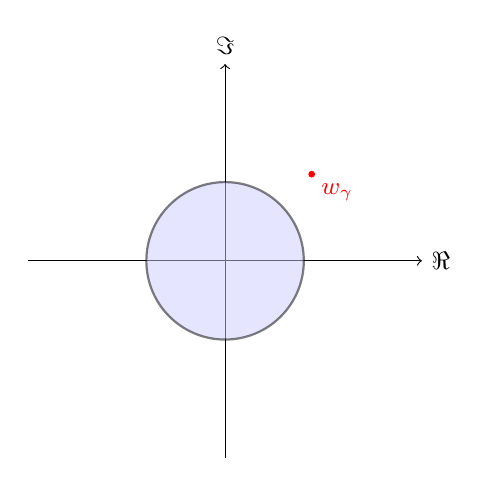
\begin{tikzpicture}[font=\small]
    % Im, Re axes
    \draw[->] (-2.5, 0) -- (2.5, 0) node[right] {$\Re$};
    \draw[->] (0, -2.5) -- (0, 2.5) node[above] {$\Im$};
    % circle
    \draw[thick, fill=blue!20, opacity=0.5] (0, 0) circle (1);
    % w_g just outside the circle
    \filldraw[red] (1.1, 1.1) circle (1pt) node[below right] {$w_\gamma$};
\end{tikzpicture}
% Ellipise mapping
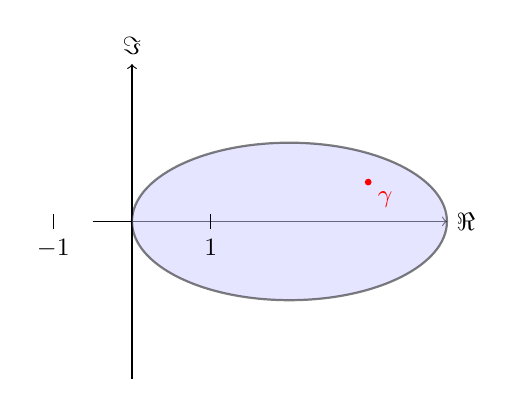
\begin{tikzpicture}[font=\small]
    % Im, Re axes
    \draw[->] (-0.5, 0) -- (4, 0) node[right] {$\Re$};
    \draw[->] (0, -2) -- (0, 2) node[above] {$\Im$};
    % Ellipse
    \draw[thick, fill=blue!20, opacity=0.5] (2, 0) ellipse (2 and 1);

    % -1, 1 ticks
    \draw (-1, 0.1) -- (-1, -0.1) node[below] {$-1$};
    \draw (1, 0.1) -- (1, -0.1) node[below] {$1$};

    % gamma just outside the ellipse
    \filldraw[red] (3, 0.5) circle (1pt) node[below right] {$\gamma$};
\end{tikzpicture}

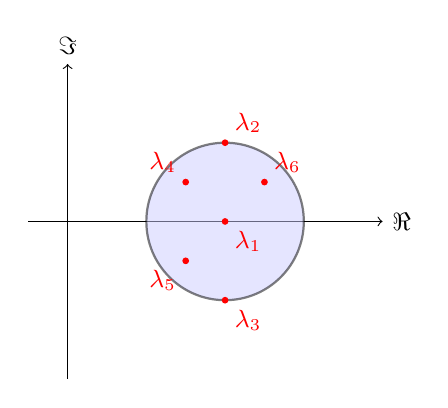
\begin{tikzpicture}[font=\small]
    % Im, Re axes
    \draw[->] (-0.5, 0) -- (4, 0) node[right] {$\Re$};
    \draw[->] (0, -2) -- (0, 2) node[above] {$\Im$};

    % Circle at (2,0) with radius 1
    \draw[thick, fill=blue!20, opacity=0.5] (2, 0) circle (1);

    % Eigenvalues
    \filldraw[red] (2, 0) circle (1pt) node[below right] {$\lambda_1$};
    \filldraw[red] (2, 1) circle (1pt) node[above right] {$\lambda_2$};
    \filldraw[red] (2, -1) circle (1pt) node[below right] {$\lambda_3$};
    \filldraw[red] (1.5, 0.5) circle (1pt) node[above left] {$\lambda_4$};
    \filldraw[red] (1.5, -0.5) circle (1pt) node[below left] {$\lambda_5$};
    \filldraw[red] (2.5, 0.5) circle (1pt) node[above right] {$\lambda_6$};
\end{tikzpicture}

Let $\lambda_i \in \mathrm{E}$ for $i = 1, \ldots, n$, where $\mathrm{E}$ is a closed ellipse, and $D_\rho := \{w \in \mathbb{C} : |w| = \rho\}$.

We search for some $p^\star$ solving the min-max problem:
\[
    \min_{\substack{p \in \mathcal{P}_m \\ p(0) = 1}} \max_{\lambda_i \in \mathrm{E}} |p(\lambda)|
\]

\subsubsection{Chebyshev polynomials in $\mathbb{C}$}
let $z \in \mathbb{C}$:
\begin{align*}
    C_m(z)     & = \cosh(m \cdot \rho), \quad \rho = \cosh^{-1}(z)                 \\
    w          & = e^{\rho}                                                        \\
    C_m(z)     & = \frac{1}{2}(e^{m\rho} + e^{-m\rho}) = \frac{1}{2}(w^m + w^{-m}) \\
    C_{m+1}(z) & = 2zC_m(z) - C_{m-1}(z), \quad C_0(z) = 1, \, C_1(z) = z          \\
    z          & = \frac{1}{2}(w + w^{-1})
\end{align*}

\begin{lemma}{Zarantonello}{}
    Let $\gamma \in \mathbb{C}$, $|\gamma| > \rho$, then:
    \[
        \min_{\substack{p \in \mathcal{P}_m \\ p(\gamma) = 1}} \max_{w \in D_\rho} = \left(\frac{\rho}{|\gamma|}\right)^m
    \]
    Minimal polynomial is given by:
    \[
        p(z) = \left(\frac{z}{\gamma}\right)^m
    \]
    Max is obtained when $z = \rho$.
\end{lemma}

\paragraph{Joukowsky mapping:}
\begin{align*}
    J(w)      & = \frac{1}{2}(w + w^{-1}), \quad w \in \mathbb{C}, \, w \neq 0 \\
    J(D_\rho) & = \mathrm{E}(0,1, \frac12(\rho + \rho^{-1}))
\end{align*}
\begin{theorem}{Elman}{}
    Let $J(D_\rho) = \mathrm{E}_\rho$ and choose $\gamma$ outside $\mathrm{E}_\rho$, and let  $ w_\gamma = J^{-1}(\gamma)$ (the biggest), then:
    \begin{align*}
        \frac{\rho^m}{|w_\gamma|^m} & \leq \min_{\substack{p \in \mathcal{P}_m \\ p(\gamma) = 1}} \max_{z \in \mathrm{E}_\rho} |p(z)| \leq \frac{\rho^m + \rho^{-m}}{|w_\gamma^m + w_\gamma^{-m}|}
    \end{align*}
    Then the optimal polynomial $p^\star$ is given by:
    \[
        p^\star(w) = \frac{w^m + w^{-m}}{w_\gamma^m + w_\gamma^{-m}}, \quad w \in \mathbb{C}
    \]
    is close to our optimal polynomial when $m$ is large.
\end{theorem}

\begin{align*}
    C_m(z)                                        & = \frac{1}{2}(w^m + w^{-m}), \quad z = \frac{1}{2}(w + w^{-1})                                                               \\
    p^\star(z)                                    & = \frac{C_m(w)}{C_m(w_\gamma)}                                                                                               \\
    \hat{C}_m(z)                                  & = \frac{C_m(\frac{z - c}{d})}{C_m(-\frac{c}{d})}, \quad \mathrm{E}(c,d,a), \quad \hat{C}_m(0) = 1                            \\
    \max_{z \in \mathrm{E}(c,d,a)} |\hat{C}_m(z)| & = \frac{C_m(\frac{a}{d})}{|C_m(-\frac{c}{d})|}                                                                               \\
    \mathbf{r}_m                                  & \leq \kappa_2(X) \eta^{(m)} \|\mathbf{r}_0\|_2 = \kappa_2(X) \frac{C_m(\frac{a}{d})}{|C_m(-\frac{c}{d})|} \|\mathbf{r}_0\|_2 \\
    C_m(z)                                        & = \frac{1}{2}\left[\left(z + \sqrt{z^2 - 1}\right)^m + \left(z - \sqrt{z^2 - 1}\right)^m\right]                              \\
    \frac{C_m(\frac{a}{d})}{|C_m(-\frac{c}{d})|}  & \approx \left(\frac{a + \sqrt{a^2 - d^2}}{c + \sqrt{c^2 - d^2}}\right)^m
\end{align*}

The ellipse enclosing the eigenvalues can not include $0$, because then $p(0) = 1$ can not be satisfied.
If $a < c$, then we have convergene for sure.




